\documentclass[aspectratio=1610]{beamer}

\usetheme[titleformat=allsmallcaps]{metropolis}

% KAIST mtheme style.
\usepackage{kaist}

\usepackage{preamble}

\title{Cartesian Dualism}
\subtitle{Mind Distinct from Body}
\date{\today}
\author{Robin Eklind}
\titlegraphic{
\includegraphics[width=0.20\textwidth]{kaistgraphics/KAIST_logo_tran.png}}

\begin{document}

% --- [ Title ] ----------------------------------------------------------------

\maketitle

% --- [ Disposition ] ----------------------------------------------------------

\begin{frame}{Disposition}
	\begin{enumerate}
		\item Substance Dualism
		\item Arguments and Counter-arguments
		\item Final Thoughts
	\end{enumerate}
\end{frame}

% === [ Substance Dualism ] ====================================================

\section{Substance Dualism}

% --- [ I think, therefore I am ] ----------------------------------------------

% called all his previous beliefs into doubt,
% to find out of what he could be certain

\begin{frame}{I think, therefore I am}
	\begin{quote}
		\textit{``I can doubt the existence of my body, but because I think, I cannot doubt the existence of my mind.''}
		- René Descartes {\tiny (paraphrased)}
	\end{quote}

	\pause
	\vspace{2em}

	\textbf{``cogito'' Argument}: Since we can doubt the existence of one, but not the other, mind and body cannot be identical.

	\pause
	\vspace{2em}

	\emph{Therefore}, we are made of two fundamentally \textbf{distinct} substances:
	\begin{itemize}
		\item \alert{Res extensa}: material thing (extended in space)
		\item \alert{Res cogitans}: thinking thing
	\end{itemize}

\end{frame}

% --- [ What is a Substance? ] -------------------------------------------------

\begin{frame}{What is a Substance?}
	By definition, a \alert{substance} can exist \emph{independently} without any other substance.

	\begin{itemize}
		\pause
		\item Matter can exist without a mind (e.g. a rock).
		\pause
		\item A mind can \textit{in principle} exist without a body.
	\end{itemize}
\end{frame}

% --- [ Where is the Mind? ] ---------------------------------------------------

\begin{frame}{Where is the Mind?}
	Nowadays considered a historical anecdote, René Descartes believed the \alert{pineal gland} to the \textit{principal seat of the soul}, through which the mind interacted with the body.

	\begin{figure}
		\centering
		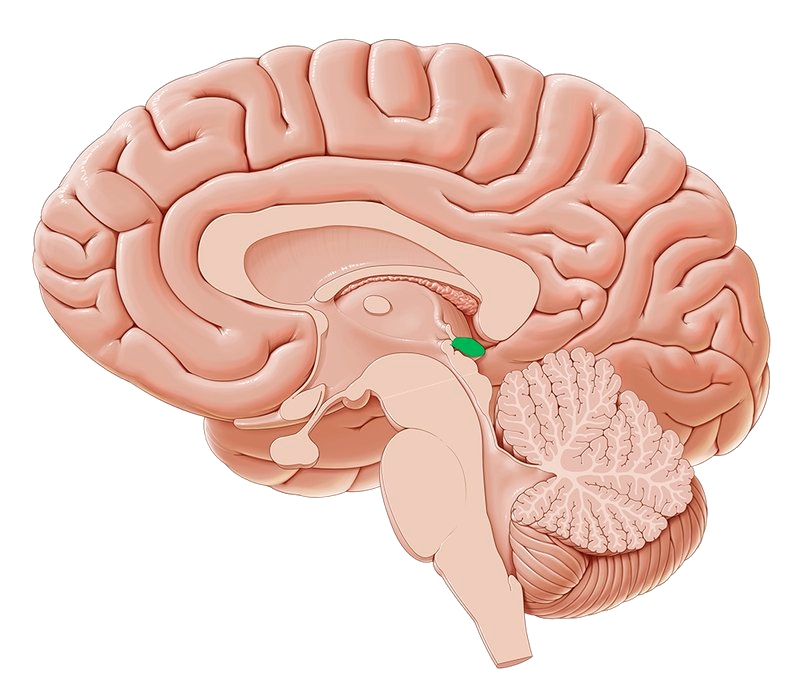
\includegraphics[height=0.55\paperheight]{inc/pineal_gland.png}
		\caption{The pineal gland of the brain.}
	\end{figure}
\end{frame}

% === [ Arguments and Counter-arguments ] ======================================

\section{Arguments and Counter-arguments}

% --- [ The Masked Person Phallacy ] -------------------------------------------

\begin{frame}{The Masked Person Phallacy}
	% reminder.
	\textbf{``cogito'' Argument}: Since we can doubt the existence of one (body), but not the other (mind), mind and body cannot be identical.

	\pause
	\vspace{2em}

	\textbf{``cogito'' Counter-argument}: \textit{The Masked Person Phallacy}
	\begin{itemize}
		\pause
		\item Doubting the existence one thing (matter) and not the other (mind) is subjective knowledge, not objective fact. Therefore they \textit{can} still be identical.
		\pause
		\item What you know about something (epistemology) is \textit{not} a property of the thing itself.
	\end{itemize}
\end{frame}

% --- [ The Pairing Problem ] --------------------------------------------------

\begin{frame}{The Pairing Problem}
	Imagine two bodies, $A$ and $B$, and a mind, $M$. How is $M$ paired with a specific body, say $A$? This is the \alert{pairing problem}.

	\pause
	\vspace{2em}

	The issue lies in the fact that \textit{res cogitans} is non-physical and has no spatial properties. How can it then be paired with a specific body?
\end{frame}

% --- [ Problem of Causal Interaction ] ----------------------------------------

\begin{frame}{Problem of Causal Interaction}
	If the mind is purly non-physical, how can it affect the physical world? This is the \alert{problem of causal interaction}.

	How can something without physical properties have physical effect?
\end{frame}

% === [ Final Thoughts ] =======================================================

\section{Final Thoughts}

% --- [ Definition of Mind? ] --------------------------------------------------

\begin{frame}{Definition of Mind?}
	It seems there is no consitent and generally agreed upon definition of the \alert{mind}.

	\pause
	\vspace{2em}

	\begin{itemize}
		\item Some definitions of the mind include every aspect of cognitive capability.
		\pause
		\item Others only include the percept or \alert{qualia} of our conscious experience.
	\end{itemize}

	\pause
	\vspace{2em}

	Without a unified definition, evaluating different philosophical frameworks and ideas becomes rather futile.
\end{frame}

% === [ Questions ] ============================================================

\begin{frame}[standout]
	Questions?
\end{frame}

\end{document}
